\section{Protocoles de la couche liaison de données}

\begin{frame}[fragile]
	\frametitle{Protocoles de la couche liaison de données}
\begin{center}
	\Huge{\bf\color{blue}Protocoles de la couche liaison de données}
\end{center}
\begin{flushright}
\end{flushright}
\end{frame}

\begin{frame}[fragile]
  \frametitle{ Protocoles de la couche de liaison}
\begin{itemize}
	\item Au niveau de la couche physique, ce sont des \textbf{bits} qui circulent sur un support
	\item Au niveau de la couche liaison de données, ce sont des \textbf{trames} qui circulent
	\item Une trame est un ensemble de bits qui encapsule un paquet (éventuellement découpé) de la couche réseau
\end{itemize}
\begin{center}
	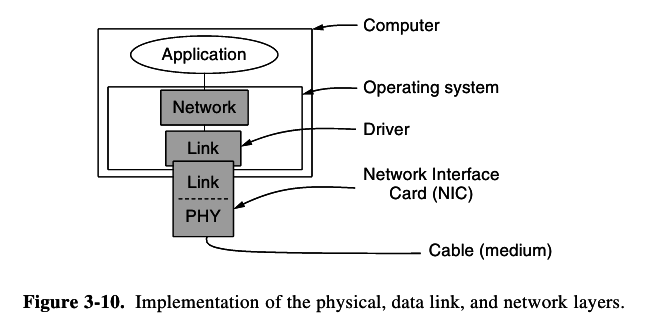
\includegraphics[width=.53\linewidth]{img/3-10.png}
	\par{\scriptsize Image de [Tanenbaum]} 
\end{center}
\end{frame}

\begin{frame}[fragile]
  \frametitle{Protocoles de la couche de liaison}
{\large\bf Protocole simplex utopique}
\begin{center}
	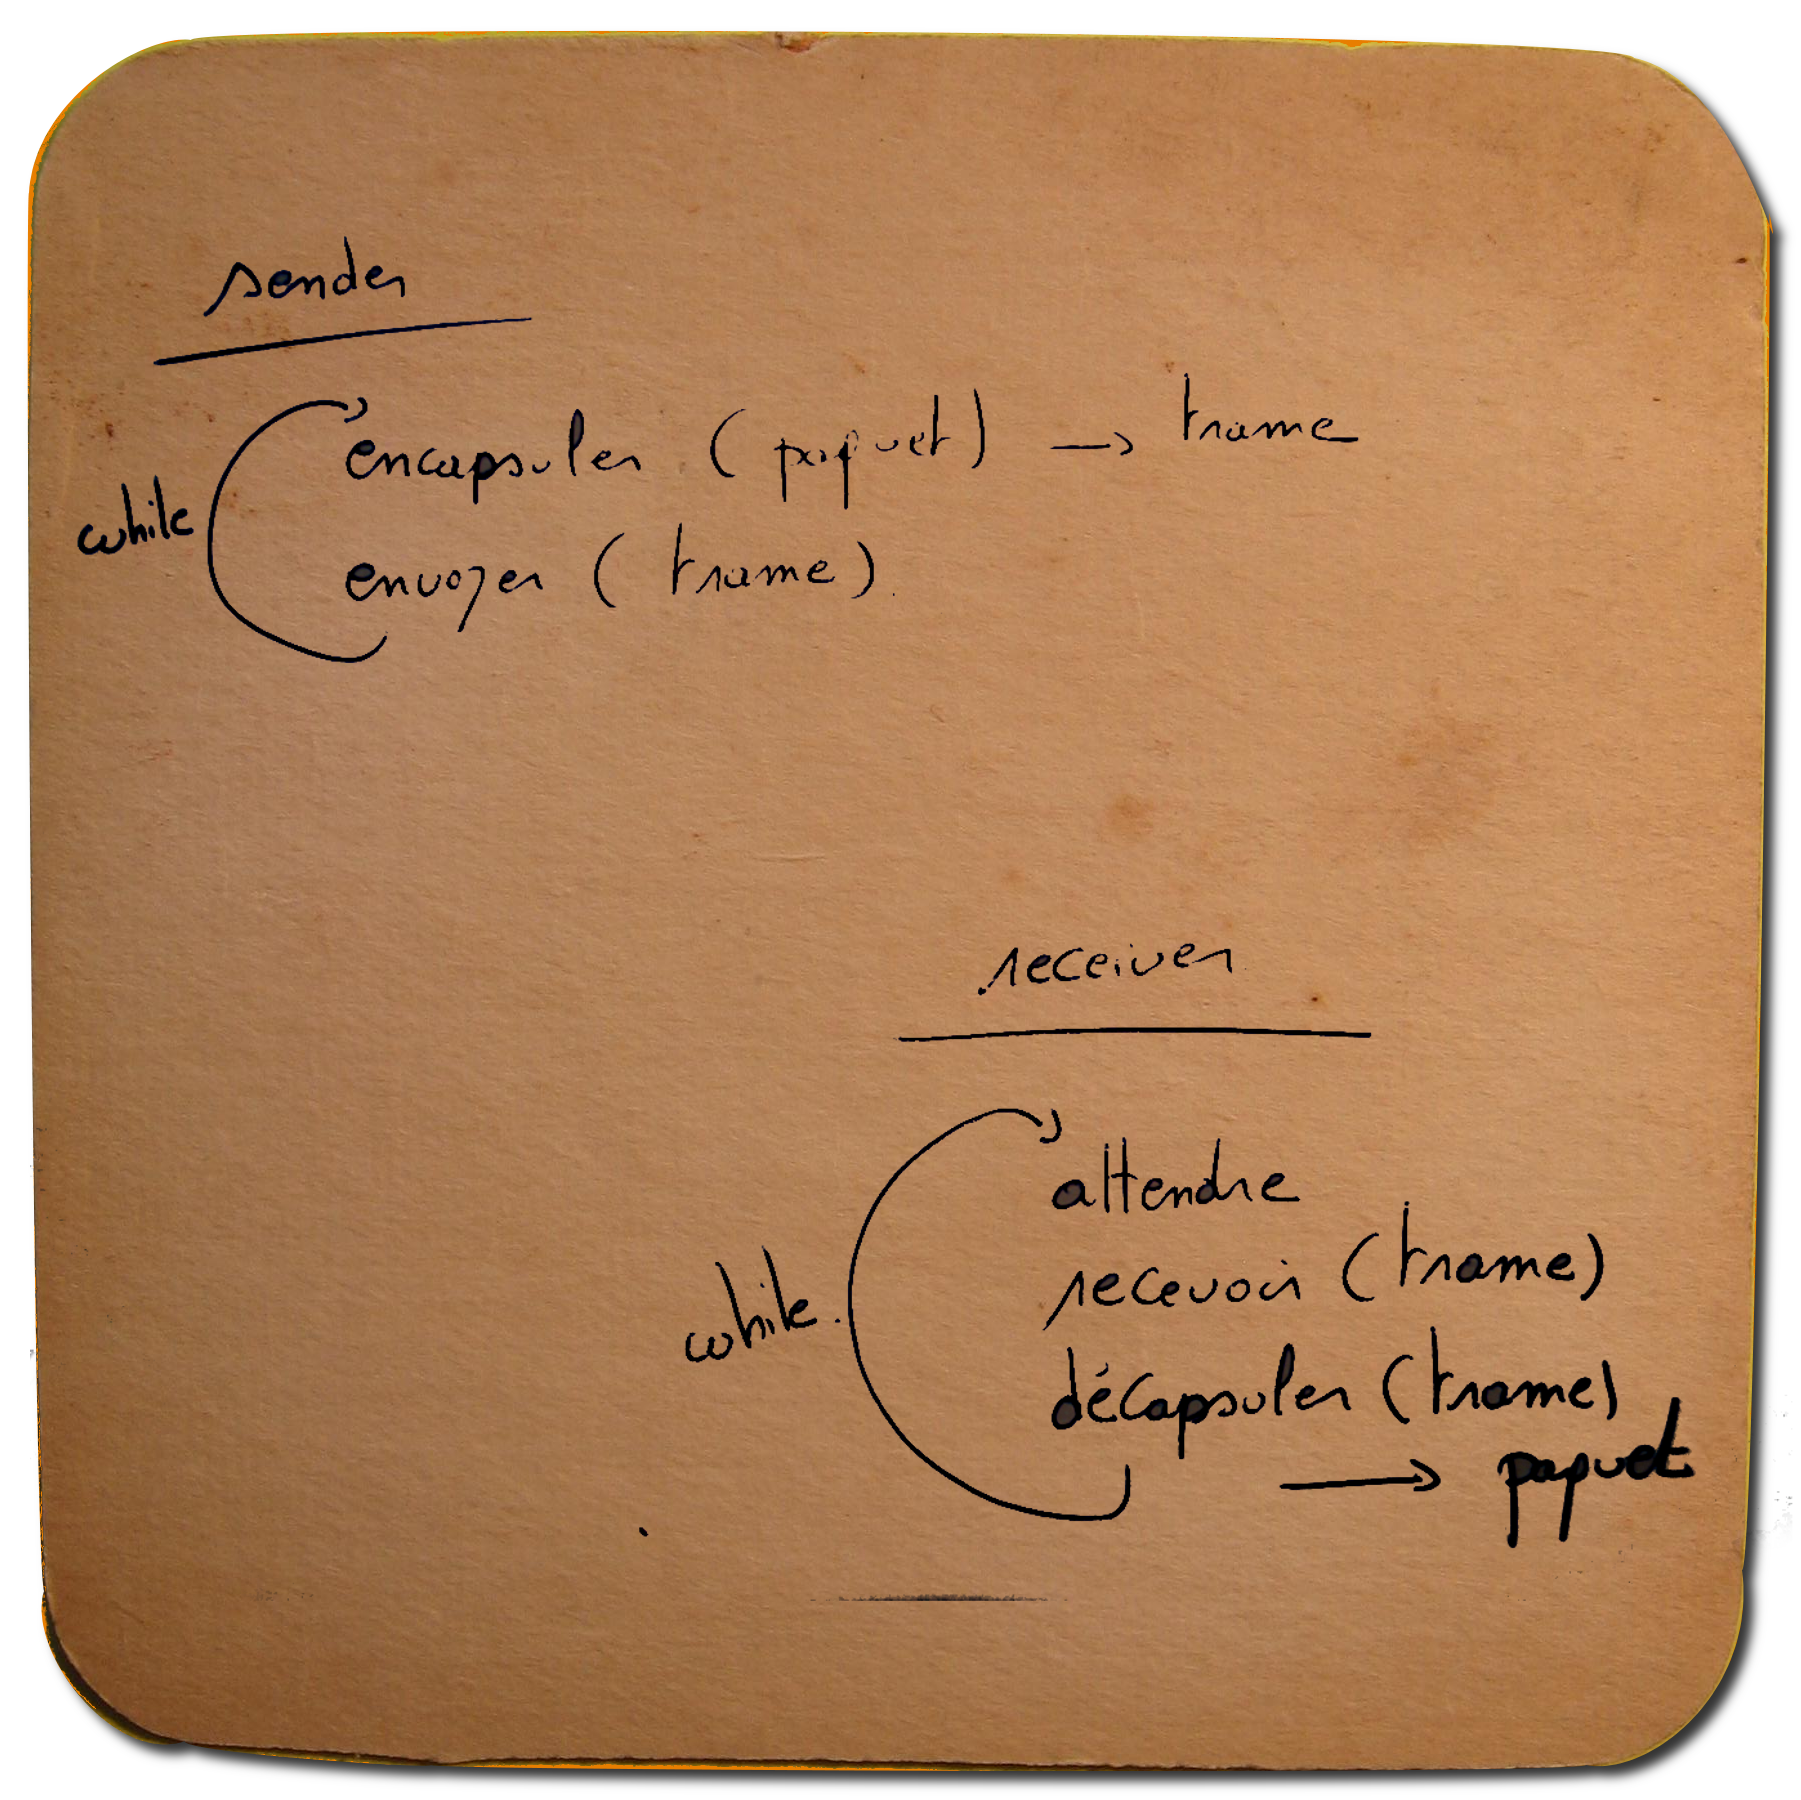
\includegraphics[width=.4\linewidth]{img/sousbock-protocole-1.png}
	\par{\scriptsize Image de [Tanenbaum]} 
\end{center}
\begin{itemize}
	\item pas de contrôle de flux (risque d'inondation)
	\item pas de correction d'erreurs
	\item pas de gestion de perte ou de trames erronées
\end{itemize}
\end{frame}

\begin{frame}[fragile]
  \frametitle{ Protocoles de la couche de liaison}
\begin{itemize}
	\item Trivialement, les trames sont envoyées en continu mais
	\begin{itemize}
		\item le débit est limité
		\item le délai de propagation est non nul
		\item des erreurs de transmission peuvent survenir
	\end{itemize}
\end{itemize}
\begin{center}
	\bf Comment résoudre ces problèmes ?
\end{center}
\end{frame}

%\begin{frame}[fragile]
%  \frametitle{Protocoles de la couche de liaison}
%\begin{itemize}
%\item Protocole simplex, stop and wait, sans bruit
%\item Protocole simplex, stop and wait, canal bruité
%\item Protocoles avec fenêtre d'anticipation
%\end{itemize}
%\end{frame}

